\documentclass[12pt]{beamer}
\usepackage{../Estilos/BeamerMAF}
\input{../Preambulos/preambulo_Beamer_Warsaw_seahorse}

\setbeamercolor{section in foot}{bg=alizarin, fg=white}
\setbeamercolor{subsection in foot}{bg=brown, fg=white}
\setbeamercolor{date in foot}{bg=goldenrod, fg=white}

\makeatletter
\setbeamertemplate{footline}
{
  \leavevmode%
  \hbox{%
  \begin{beamercolorbox}[wd=.333333\paperwidth,ht=2.25ex,dp=1ex,center]{section in foot}%
    \usebeamerfont{section in foot} \insertsection
  \end{beamercolorbox}%
  \begin{beamercolorbox}[wd=.333333\paperwidth,ht=2.25ex,dp=1ex,center]{subsection in foot}%
    \usebeamerfont{subsection in foot}  \insertsubsection
  \end{beamercolorbox}%
  \begin{beamercolorbox}[wd=.333333\paperwidth,ht=2.25ex,dp=1ex,right]{date in head/foot}%
    \usebeamerfont{date in head/foot} \insertshortdate{} \hspace*{2em}
    \insertframenumber{} / \inserttotalframenumber \hspace*{2ex} 
  \end{beamercolorbox}}%
  \vskip0pt%
}
\makeatother

\date{24 de febrero de 2022}
\title{Ondas transversales en coord. cilíndricas}
\subtitle{La física y la geometría}
\begin{document}
\maketitle
\fontsize{14}{14}\selectfont
\spanishdecimal{.}

\section*{Contenido}
\frame[allowframebreaks]{\frametitle{Contenido} \tableofcontents[currentsection, hideallsubsections]}

\section{Marco de referencia.}
\frame{\tableofcontents[currentsection, hideothersubsections]}
\subsection{Guías de ondas.}

\begin{frame}
\frametitle{¿Qué es una guía de onda?}
Una guía de ondas es una estructura elaborada por conductores, dieléctricos, o una combinación de éstos, cuenta con una sección recta constante en una dirección que permite propagar o guiar ondas electromagnéticas ya sea en su interior, en sus proximidades o en ambas regiones.
\end{frame}
\begin{frame}
\frametitle{Una onda electromagnética}
\begin{figure}[H]
    \centering
    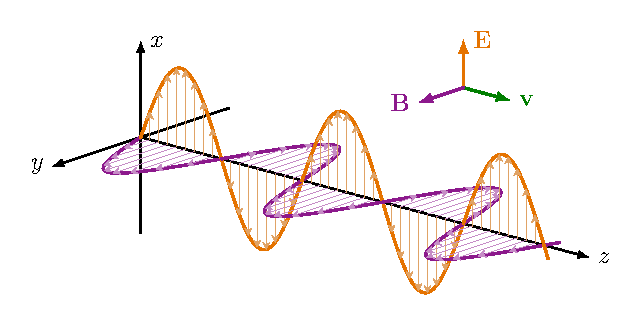
\includegraphics[scale=1]{Imagenes/Onda_Electromagnetica.eps}
    \caption{Onda electromagnética.}
\end{figure}
\end{frame}
\begin{frame}
\frametitle{Tipos de guía de onda}
La geometría de la guía de onda queda determinada por la forma y frecuencia de las ondas que deben propagar, como se aprecia en la figura (\ref{fig:figura_01}):
\end{frame}
\begin{frame}
\frametitle{Tipos de guía de onda}
\begin{figure}[H]
    \centering
    \includegraphics[scale=0.15]{Imagenes/Tubos_Guias_Onda.jpg}
    \caption{Tres tipos de guías de onda: elíptico, rectangular y circular.}
    \label{fig:figura_01}
\end{figure}
\end{frame}
\begin{frame}
\frametitle{Usos de las guía de onda}
Las guías de onda son adecuadas para transmitir señales debido a su bajas pérdidas.
\\
\bigskip
\pause
Por ello, se usan en microondas, a pesar de su ancho de banda limitado y volumen, mayor que el de líneas impresas o coaxiales para la misma frecuencia.
\end{frame}
\begin{frame}
\frametitle{Guía de onda coaxial}
En la figura (\ref{fig:figura_02}) se muestra un esquema de una guía de onda de tipo coaxial.
\begin{figure}[H]
    \centering
    \includegraphics[scale=1.4]{Imagenes/Guia_Onda_Coaxial.eps}
    \caption{Esquema de una guía de onda coaxial con radio interno $a$ y radio externo $b$.}
    \label{fig:figura_02}
\end{figure}
\end{frame}
\begin{frame}
\frametitle{Estudiando los campos en las guías}
Las ecuaciones generales que describen el comportamiento de los campos que se propagan en las guías de onda, son soluciones generales de las ecuaciones de Maxwell.
\end{frame}
\begin{frame}
\frametitle{Consideraciones}
Como consideraciones debemos de tomar en cuenta que:
\setbeamercolor{item projected}{bg=blue!70!black,fg=yellow}
\setbeamertemplate{enumerate items}[circle]
\begin{enumerate}[<+->]
\item Las ondas se generan únicamente con señales senoidales.\item Las guías de onda son infinitamente largas.
\item La dirección de propagación de los campos está en la dirección $z$, según los ejes de coordenadas cartesianas o cilíndricas.
\end{enumerate}
\end{frame}
\begin{frame}
\frametitle{Las soluciones}
Estas ecuaciones tienen soluciones múltiples, o modos.
\\
\bigskip
\pause
Los modos de propagación dependen de la longitud de onda, de la polarización y de las dimensiones de la guía. \pause El \emph{modo longitudinal} de una guía de onda es un tipo particular de onda estacionaria formado por ondas confinadas en la cavidad.
\end{frame}

\subsection{Modos de Propagación.}

\begin{frame}
\frametitle{Clasificando los modos de propagación}
Los modos transversales se clasifican en distintos tipos:
\setbeamercolor{item projected}{bg=blue!70!black,fg=yellow}
\setbeamertemplate{enumerate items}[circle]
\begin{enumerate}[<+->]
\item Modo TE (Transversal eléctrico), la componente de $\vb{E}$ en la dirección de propagación es nula.
\item Modo TM (Transversal magnético), la componente de $\vb{B}$ en la dirección de propagación es nula.
\seti
\end{enumerate}
\end{frame}
\begin{frame}
\frametitle{Clasificando los modos de propagación}
\setbeamercolor{item projected}{bg=blue!70!black,fg=yellow}
\setbeamertemplate{enumerate items}[circle]
\begin{enumerate}[<+->]
\conti
\item Modos TEM (Transversal electromagnético), la componente tanto del $\vb{E}$ como de $\vb{B}$ en la dirección de propagación es nula.
\item Modos híbridos: son los que sí tienen componente en la dirección de propagación tanto en el campo eléctrico como en el de inducción magnética.
\end{enumerate}
\end{frame}

\section{El Laplaciano de una función vectorial.}
\frame{\tableofcontents[currentsection, hideothersubsections]}
\subsection{Definición.}

\begin{frame}
\frametitle{Definiendo el Laplaciano de un vector}
El Laplaciano de un campo vectorial $\vb{V}$, que se expresa como $\laplacian{\vb{V}}$, se define como:
\pause
\begin{align*}
\laplacian{\vb{V}} = \grad{\div{\vb{V}}} - \curl{\curl{\vb{V}}}
\end{align*}
\end{frame}
\begin{frame}
\frametitle{El operador para problemas de guías de onda}
En problemas de guías de ondas circulares y resonadores de cavidades cilíndricas, el Laplaciano vectorial en coordenadas cilíndricas circulares es:
\pause
\begin{align*}
\laplacian{\va{V}} \Rightarrow \begin{cases}
\laplacian{V_{\rho}} = \laplacian{V_{\rho}} - \dfrac{1}{\rho} V_{\rho} - \dfrac{2}{\rho^{2}} \displaystyle \pdv{V_{\varphi}}{\varphi} \\[0.75em]
\laplacian{V_{\varphi}} = \laplacian{V_{\varphi}} - \dfrac{1}{\rho} V_{\varphi} - \dfrac{2}{\rho^{2}} \displaystyle \pdv{V_{\rho}}{\varphi} \\[0.75em]
\laplacian{V_{z}} = \laplacian{V_{z}}
\end{cases}
\end{align*}
\end{frame}
\begin{frame}
\frametitle{Caso particular}
En donde podemos notar que el Laplaciano de una función escalar es similar a la componente $z$ del Laplaciano de un campo vectorial.
\end{frame}

\section{Enunciado del ejercicio.}
\frame{\tableofcontents[currentsection, hideothersubsections]}
\subsection{Planteamiento.}

\begin{frame}
\frametitle{El enunciado del problema a resolver}
Una onda electromagnética transversal en una guía de onda coaxial tiene un campo eléctrico $\vb{E} = \vb{E} (\rho, \varphi) \, \exp(i [k z - \omega t])$ \pause y un campo de inducción magnética $\vb{B} = \vb{B} (\rho, \varphi) \, \exp(i [k z - \omega t])$.
\\
\bigskip
\pause
Como la onda es transversal, ni $\vb{E}$ ni $\vb{B}$ tienen componente $z$.
\end{frame}
\begin{frame}
\frametitle{El enunciado del problema a resolver}
Los dos campos satisfacen la ecuación de Laplace vectorial:
\pause
\begin{align*}
\laplacian{\vb{E} (\rho, \varphi)} &= 0 \\[0.5em]
\laplacian{\vb{B} (\rho, \varphi)} &= 0
\end{align*}
\end{frame}
\begin{frame}
\frametitle{Incisos a resolver}
\setbeamercolor{item projected}{bg=blue!70!black,fg=yellow}
\setbeamertemplate{enumerate items}[circle]
\begin{enumerate}[<+->]
\item Demuestra que:
\begin{align*}
\vb{E} &= \vu{\bm{\rho}} \, \bigg( \dfrac{a}{\rho} \bigg) E_{0} \, \exp(i [k z - \omega t]) \\[0.5em]
\vb{B} &= \vu{\bm{\varphi}} \, \bigg( \dfrac{a}{\rho} \bigg) B_{0} \, \exp(i [k z - \omega t])
\end{align*}
son soluciones. Considera que $a$ es el radio del conductor interno y $E_{0}$ y $B_{0}$ son amplitudes constantes.
\seti
\end{enumerate}
\end{frame}
\begin{frame}
\frametitle{Incisos a resolver}
\setbeamercolor{item projected}{bg=blue!70!black,fg=yellow}
\setbeamertemplate{enumerate items}[circle]
\begin{enumerate}[<+->]
\conti
\item Suponiendo que hay vacío dentro de la guía de onda, verifica que las ecuaciones de Maxwell se satisfacen con:
\begin{align*}
\dfrac{B_{0}}{E_{0}} = \dfrac{k}{\omega} = \mu_{0} \varepsilon_{0} \bigg( \dfrac{\omega}{k} \bigg) = \dfrac{1}{c}
\end{align*}
\end{enumerate}
\end{frame}

\section{Solución.}
\frame{\tableofcontents[currentsection, hideothersubsections]}
\subsection{Inciso 1)}

\begin{frame}
\frametitle{Identificando lo necesario}
Para $\vb{E} (\rho, \varphi)$, la ecuación relevante es la que contiene la componente $\rho$ del vector Laplaciano, ya que las otras componentes se anulan.
\end{frame}
\begin{frame}
\frametitle{Para el campo eléctrico}
\begin{eqnarray*}
\begin{aligned}
\laplacian{E} &= \laplacian{E_{\rho}} - \dfrac{1}{\rho^{2}} E_{\rho} = \\[0.5em] \pause
&= \dfrac{1}{\rho} \pdv{\rho} \bigg( \rho \pdv{E_{\rho}}{\rho} \bigg) - \dfrac{1}{\rho^{2}} E_{\rho} = \\[0.5em] \pause
&= \dfrac{1}{\rho} \pdv{\rho} \bigg( - \dfrac{a}{\rho} E_{0} \bigg) - \dfrac{a}{\rho^{3}} E_{0} = \\[0.5em] \pause
&= \dfrac{a}{\rho^{3}} E_{0} - \dfrac{a}{\rho^{3}} E_{0} = 0
\end{aligned}
\end{eqnarray*}
\end{frame}
\begin{frame}
\frametitle{Para el campo de inducción magnética}
Para $\vb{B} (\rho, \varphi)$, la ecuación relevante es la que contiene la componente $\varphi$ del vector Laplaciano:
\pause
\begin{eqnarray*}
\begin{aligned}
\laplacian{\vb{B}} &= \laplacian{B_{}\varphi} - \dfrac{1}{\rho^{2}} B_{\varphi} = \\[0.5em] \pause
&= \dfrac{1}{\rho^{2}} B_{\varphi} - \dfrac{1}{\rho^{2}} B_{\varphi} = 0
\end{aligned}
\end{eqnarray*}
\end{frame}

\subsection{Inciso 2)}
\begin{frame}
\frametitle{Resolviendo el inciso 2)}
Para verificar que las soluciones satisfacen las ecuaciones de Maxwell, debemos de expresar tanto la divergencia como el rotacional de $\vb{E}$ y $\vb{B}$.
\end{frame}
\begin{frame}
\frametitle{La divergencia del campo eléctrico}
Para el campo eléctrico $\vb{E}$:
\pause
\begin{eqnarray*}
\begin{aligned}
0 &= \div{\vb{E}} = \dfrac{1}{\rho} \pdv{\rho} \bigg( \rho E_{\rho} \bigg) + \dfrac{1}{\rho} \pdv{E_{\rho}}{\varphi} + \pdv{E_{z}}{z} = \\[0.5em] \pause
&= \dfrac{1}{\rho} \pdv{\rho} \bigg( a E_{0} \bigg) = 0
\end{aligned}
\end{eqnarray*}
\end{frame}
\begin{frame}
\frametitle{La divergencia del campo de inducción magnética}
Para el campo de inducción magnética $\vb{B}$:
\pause
\begin{eqnarray*}
\begin{aligned}
0 &= \div{\vb{B}} = \dfrac{1}{\rho} \pdv{\rho} \bigg( \rho B_{\rho} \bigg) + \dfrac{1}{\rho} \pdv{B_{\rho}}{\varphi} + \pdv{B_{z}}{z} = \\[0.5em] \pause
&= \dfrac{1}{\rho} \pdv{\rho} \bigg( a B_{0}\bigg) = 0
\end{aligned}
\end{eqnarray*}
\end{frame}
\begin{frame}
\frametitle{El rotacional del campo eléctrico}
Para el rotacional de $\vb{E}$:
\pause
\begin{eqnarray*}
\begin{aligned}
0 &= \curl{\vb{E}} + \pdv{\vb{B}}{t} = \\[0.5em] \pause
&= \dfrac{1}{\rho} \mqty|
\vu{\bm{\rho}} & \rho \, \vu{\bm{\varphi}} & \vu{z} \\[0.5em] 
\displaystyle \pdv{\rho} & \displaystyle  \pdv{\varphi} & \displaystyle \pdv{z} \\[0.5em] 
E_{\rho} & E_{\varphi} & E_{z} | + \pdv{\vb{B}}{t} =
\end{aligned}
\end{eqnarray*}
\end{frame}
\begin{frame}
\frametitle{El rotacional del campo eléctrico}
\begin{eqnarray*}
\begin{aligned}
0 &= \curl{\vb{E}} + \pdv{\vb{B}}{t} = \\[0.5em] \pause
&= \dfrac{1}{\rho} \bigg[ - \vu{\bm{\varphi}} \, i \, k \, a \, E_{0} \, \exp(i [k z - \omega t]) - 0 \bigg] + \\[0.5em] \pause
&+ \vb{\bm{\varphi}} \, (- i \omega) \dfrac{a}{\rho} \, B_{0} \, \exp(i [k z - \omega t]) = \\[0.5em] \pause
&= \vb{\bm{\varphi}} \, \dfrac{i \, a}{\rho} \, \exp(i [k z - \omega t]) \bigg[ k \, E_{0} - \omega \, B_{0} \bigg]
\end{aligned}
\end{eqnarray*}
\end{frame}
\begin{frame}
\frametitle{Condición necesaria}
Para que se cumpla la igualdad, debe ocurrir:
\pause
\begin{eqnarray*}
\begin{aligned}
k \, E_{0} - \omega \, B_{0} &= 0 \\[0.5em] \pause
\Rightarrow \hspace{0.2cm} k \, E_{0} &= \omega \, B_{0} \\[0.5em] \pause
\Rightarrow \hspace{0.2cm} \dfrac{B_{0}}{E_{0}} &= \dfrac{k}{\omega}
\end{aligned}
\end{eqnarray*}
que es la condición que se señaló en el enunciado.
\end{frame}
\begin{frame}
\frametitle{El rotacional del campo de inducción magnética}
Para el campo de inducción magnética $\vb{B}$:
\pause
\begin{eqnarray*}
\begin{aligned}
0 &= \curl{\vb{B}} - \mu_{0} \, \varepsilon_{0} \, \pdv{\vb{E}}{t} = \\[0.5em] \pause
&= \dfrac{1}{\rho} \mqty|
\vu{\bm{\rho}} & \rho \, \vu{\bm{\varphi}} & \vu{z} \\[0.5em]
\displaystyle \pdv{\rho} & \displaystyle  \pdv{\varphi} & \displaystyle \pdv{z} \\[0.5em]
B_{\rho} & B_{\varphi} & B_{z} | - \mu_{0} \, \varepsilon_{0} \, \pdv{\vb{E}{t}} = 
\end{aligned}
\end{eqnarray*}
\end{frame}
\begin{frame}
\frametitle{El rotacional del campo de inducción magnética}
\begin{eqnarray*}
\begin{aligned}
0 &= \curl{\vb{B}} - \mu_{0} \, \varepsilon_{0} \, \pdv{\vb{E}}{t} = \\[0.5em] \pause
&= \dfrac{1}{\rho} \bigg[ 0 - \vu{\bm{\rho}} \, i \, k \, a \, B_{0} \, \exp(i [k z - \omega t]) \bigg] + \\[0.5em] \pause
&- \vu{\bm{\rho}} \, \mu_{0} \, \varepsilon_{0} (- i \, \omega) \dfrac{a}{\rho} E_{0} \, \exp(i [k z - \omega t]) = \\[0.5em] \pause
&= \vu{\bm{\rho}} \, \dfrac{i \, a}{\rho} \, \exp(i [k z - \omega t]) \, \bigg( - k \, B_{0} + \mu_{0} \, \varphi_{0} \, E_{0} \bigg)
\end{aligned}
\end{eqnarray*}
\end{frame}
\begin{frame}
\frametitle{Condición necesaria}
Para que se cumpla la igualdad, debe de ocurrir que:
\pause
\begin{eqnarray*}
- k \, B_{0} + \mu_{0} \, \varphi_{0} \, E_{0} &= 0 \\[0.5em] \pause
\Rightarrow \hspace{0.3cm} k \, B_{0} = \mu_{0} \, \varphi_{0} \, E_{0} \\[0.5em] \pause
\Rightarrow \hspace{0.3cm} \dfrac{B_{0}}{E_{0}} = \dfrac{\mu_{0} \, \varphi_{0} \, \omega}{k}
\end{eqnarray*}
tal como se indicó en el enunciado del ejercicio. $\qed$
\end{frame}
\end{document}